% !TEX program = xelatex
\documentclass[]{article}
\usepackage{commons/course}

\begin{document}
\printheader

\section{}
بله این تابع نیز مقاوم است. همان طور که در صورت سوال هم گفته شد کافی است که اثبات کنیم که نمی‌توانیم
دو ورودی پیدا کنیم به صورتی که
$H'(x) = H'(y)$ و $x \neq y$.
همان طور که صورت سوال نیز گفته است
$H'(x) = H(H(x))$
است و می‌دانیم که
$H$
در برابر تصادم مقاوم است. پس برای اینکه
$H'(x) = H'(y)$
باشد باید عملا
$H(x) = H(y)$
باشد که می‌دانیم که از لحاظ محاسباتی غیر ممکن است پس این تابع نیز مقاوم است.
\section{}
یکی از مزیت‌هایی که
\lr{CFB} و \lr{OFB}
نسبت به
\lr{CBC}
دارند این است که در
\lr{CBC}
نیاز است که حتما از
\lr{padding}
استفاده کنیم که طول ورودی بر طول بلاک بخش پذیر باشد. ولی در
\lr{CFB} و \lr{OFB}
نیازی به آن نیست. یکی از خوبی‌هایی که هر دو الگوریتم دارند این است که می‌توان آخرین بلوک آن‌ها را به عنوان یک
\lr{checksum}
در نظر گرفت ولی همین یک بدی نیز است چرا که اگر به صورت اشتباهی وسط پیام عوض شود کل پیام بعد از آن
نقطه خراب می‌شود.

\noindent
\link{https://en.wikipedia.org/wiki/Block_cipher_mode_of_operation\#CFB_compared_to_other_modes}{منبع}
\section{}
% https://d-nb.info/1206696850/34
\begin{enumerate}
    \item \begin{itemize}
        \item \textbf{بهمنی اکید:} این خاصیت بدین معنی است که اگر یک بیت از ورودی عوض شود باید تمامی بیت‌های خروجی با احتمال یک دوم تغییر کنند. (\link{https://ieeexplore.ieee.org/document/5762665}{منبع})
        \item \textbf{تمامیت:} این خاصیت نشان می‌دهد که تمامی بیت‌های خروجی به تمامی بیت‌های ورودی بستگی دارد. (\link{https://en.wikipedia.org/wiki/Completeness_(cryptography)}{منبع})
        \item \textbf{\lr{Random Cipher}:} TODO
    \end{itemize}
    \item کافی است که اینقدر تکرار و دور داشته باشیم که هرگاه هر کدام از
    $X_0$ تا $X_3$
    عوض شوند حتما کل خروجی‌ها نیز عوض می‌شوند. در ابتدا مشخص است که خود الگوریتم با یک دور خاصیت بهمنی
    را ندارد چرا که اصلا تغییر
    $X_1$
    بر روی
    $Y_3$
    تاثیری نمی‌گذارد. حال بررسی می‌کنیم که اگر دو بار تکرار انجام دهیم چه می‌شود. در اینجا متوجه می‌شیم که تغییر
    $X_3$
    بر روی
    $Y_0$
    تاثیری ندارد. (با توجه به شکل \ref{fig:generalized-feistel:2round})
    \begin{figure}
        \centering
        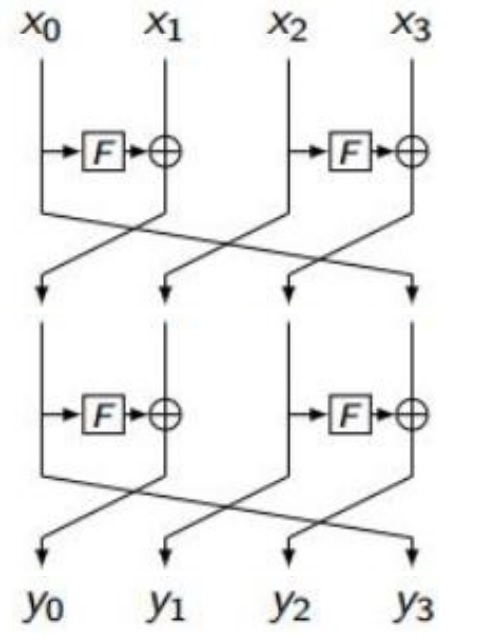
\includegraphics[scale=0.5]{pics/3-2-rounds.jpg}
        \caption{دو دور در \lr{generalized feistel}}
        \label{fig:generalized-feistel:2round}
    \end{figure}
    حال باید بررسی بکنیم که در سه دور چه اتفاقی می‌افتد. در این حالت اگر
    $X_1$
    عوض شود هیچ تغییری در
    $Y_1$
    رخ نمی‌دهد به صورت شکل
    \ref{fig:generalized-feistel:3round}.
    \begin{figure}
        \centering
        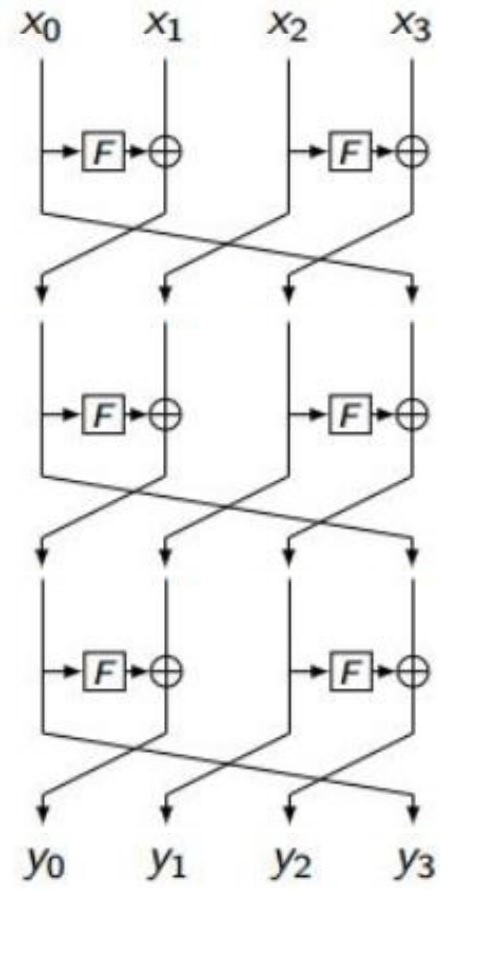
\includegraphics[scale=0.5]{pics/3-3-rounds.jpg}
        \caption{سه دور در \lr{generalized feistel}}
        \label{fig:generalized-feistel:3round}
    \end{figure}
    اما با چهار دور تمامی خورجی‌ها وابسته تمامی ورودی‌ها می‌شوند و دیگر با تغییر حتی یکی
    از ورودی‌ها تمامی خروجی‌ها عوض می‌شود. همچنین من با جست و جو در اینترنت دقیقا یک مقاله پیدا کردم
    که بر روی تعداد جایگشت‌های یک
    \lr{cipher}
    مانند این سوال کار می‌کند که در
    \link{https://d-nb.info/1206696850/34}{اینجا}
    موجود است.
\end{enumerate}
\section{}
\section{}
\section{}
\section{}
\end{document}
